\documentclass[11pt]{article}
\usepackage{preamble}
\usepackage{gset}
\def\week{4}
\def\theproblem{К\week.\arabic{problem}}
\begin{document}
\setcounter{problem}{0}
\def\theproblem{Д\week.\arabic{problem}}
{\textbf{\large Дискретная математика}\hfill \textbf{(Основной поток)}

\medskip %

\textbf{Домашнее задание \week}}

\medskip

\textbf{Дайте обоснованные ответы на следующие вопросы.}


\vspace{5mm}

\p
Функция  $f$ из множества $X$   в~множество $Y$ такова, что для
$A\subseteq X$, $B\subseteq X$ выполняется
\[
f^{-1}(f(A)) =   f^{-1}( f(B))
\]
(здесь $f^{-1}$ обозначает полный прообраз множества). Следует ли из этого равенство $A=B$?
Приведите доказательство или контрпример.
\bs
Пусть $A = \{-1\}, B = \{1\}, f = x^2$. Тогда $f^-1(f(A)) = f^-1(f(B)) \land A \neq B$
\bs 
\answer{Нет} \bs
\p  Функция  $f$ определена на множестве $A\cup B$ и принимает значения в
множестве $Y$.
Если заменить в  утверждении 
\[
f(A \sym B) \mathbin{?} f(A) \sym f(B)\qquad\text{($\sym$ обозначает симметрическую разность)}
\]
знак  $?$ на один из знаков  включения $\subseteq$ или $\supseteq$,
получится утверждение. Какие из получившихся двух утверждений верны для
любой $f$? Приведите доказательство или контрпример в каждом случае.
\[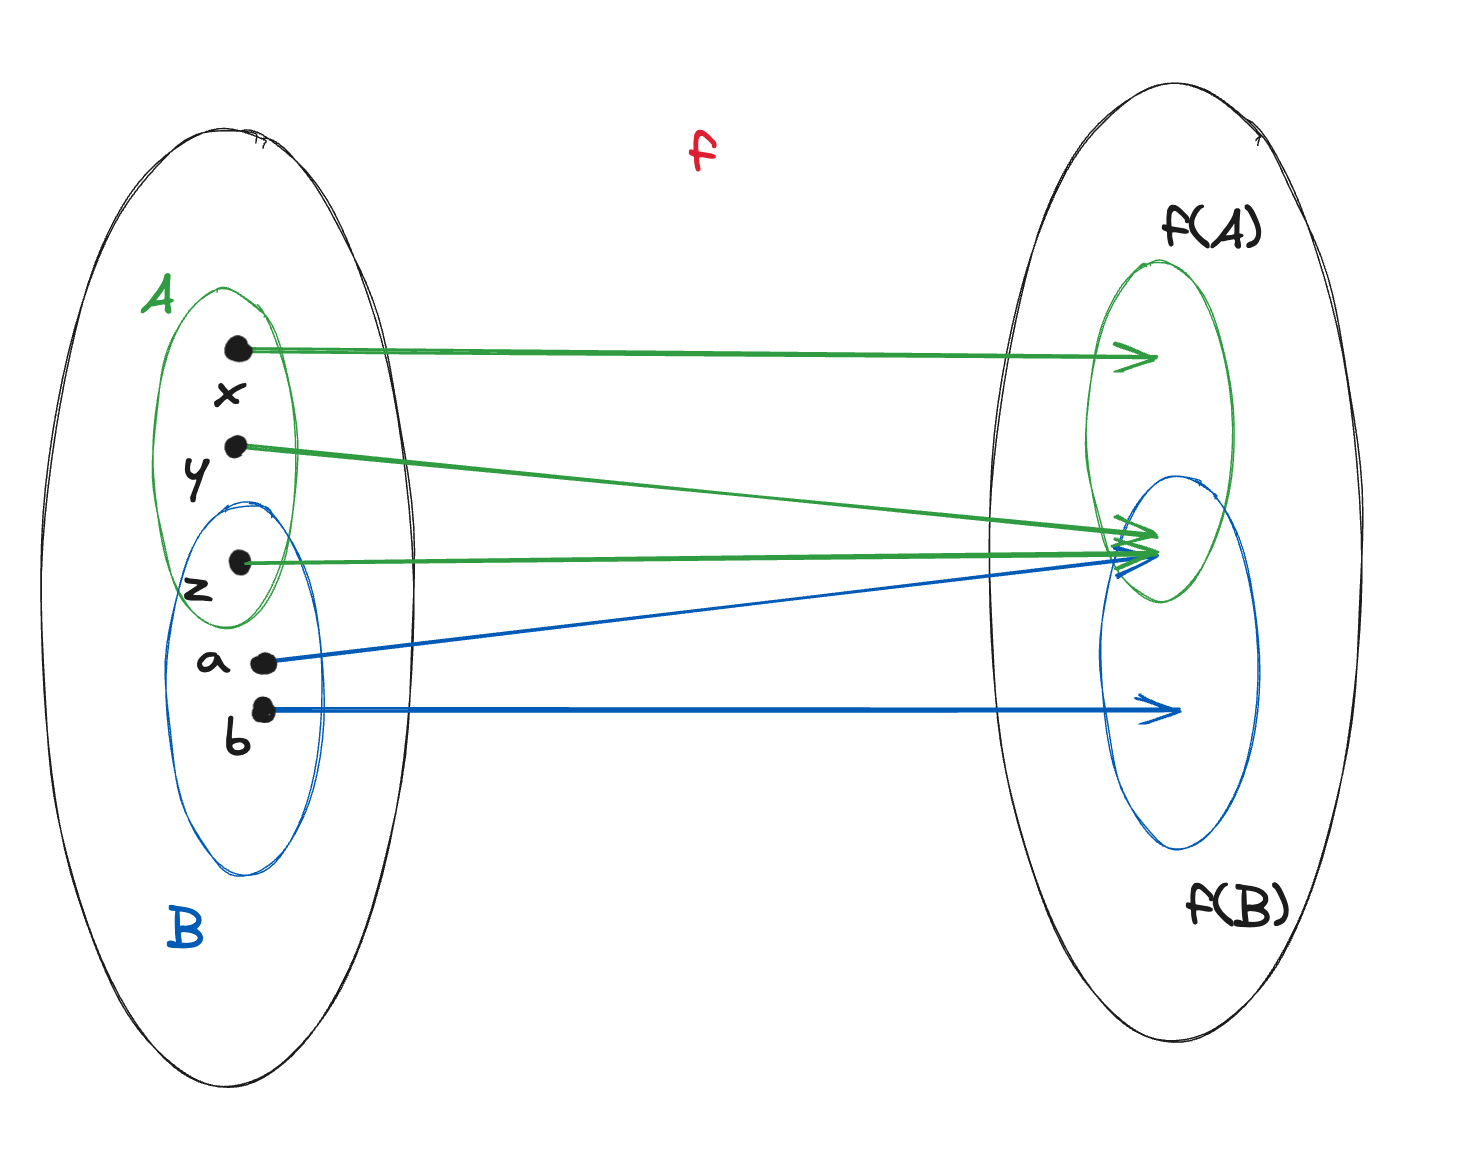
\includegraphics[width=125mm]{img4}\]
\[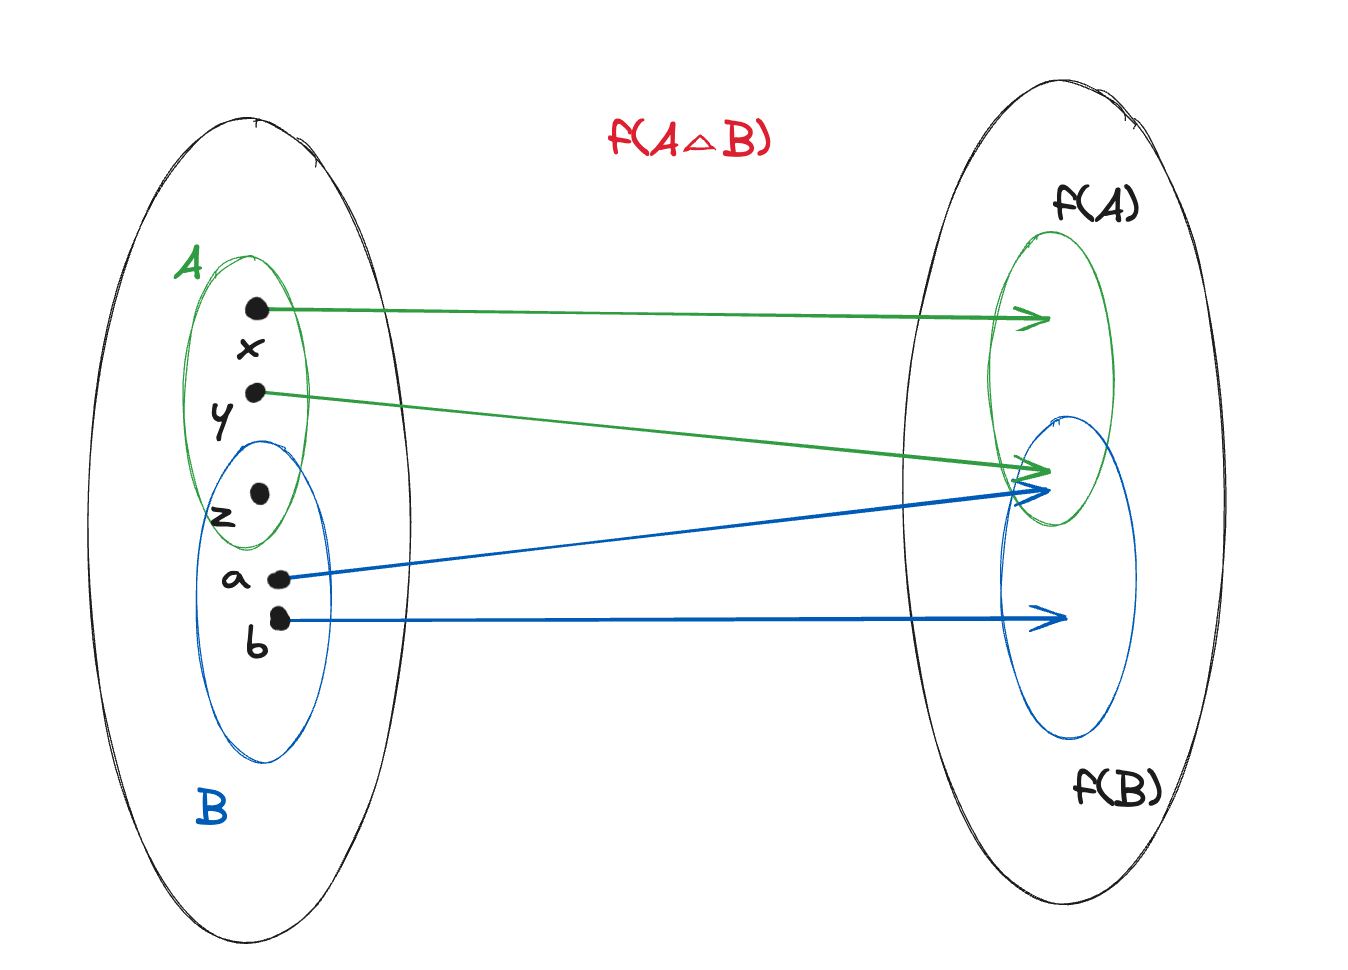
\includegraphics[width=125mm]{img2}\]
\[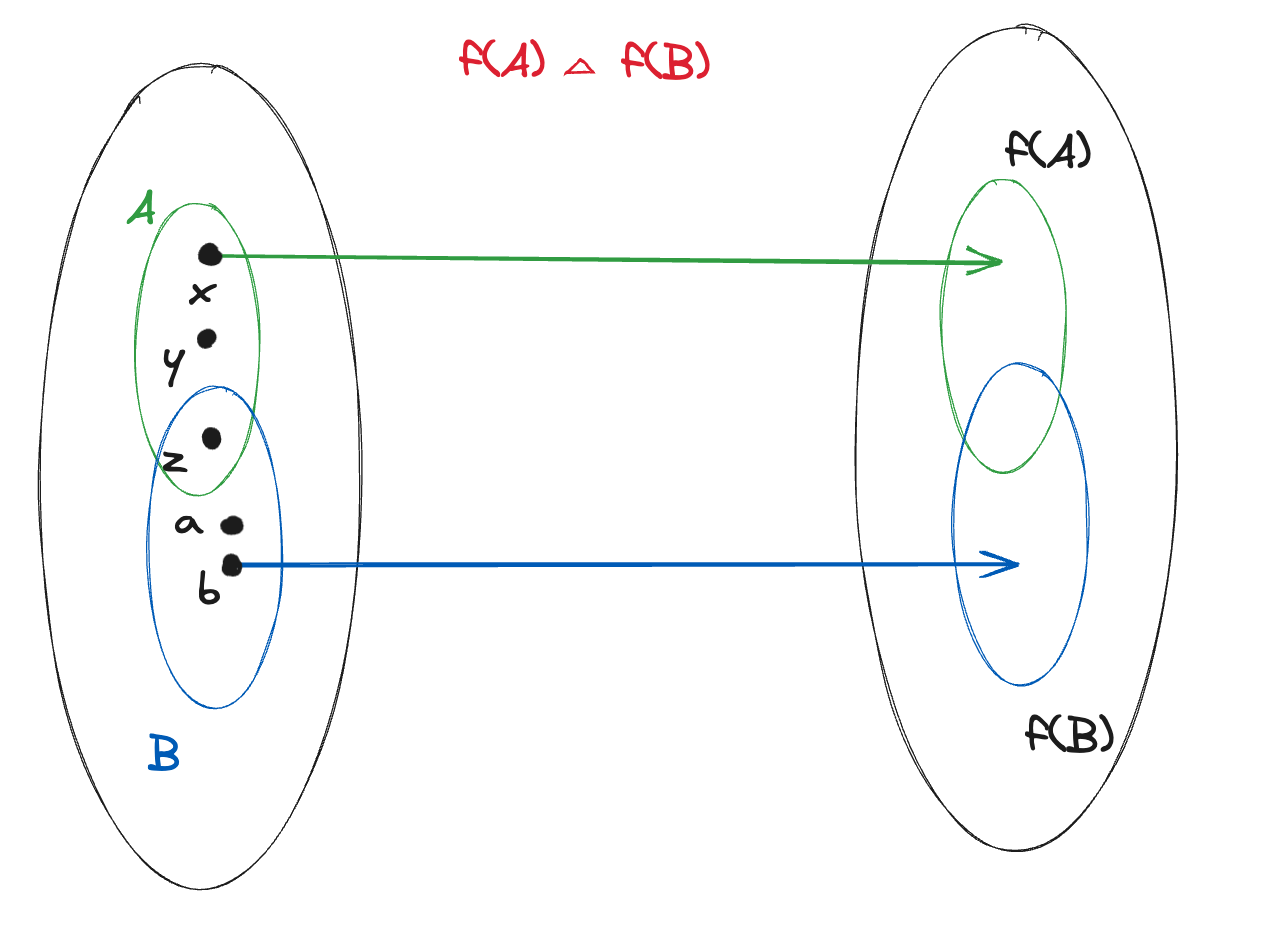
\includegraphics[width=125mm]{img3}\]
\bs
1) $f(A \sym B) \mathbin{\subseteq} f(A) \sym f(B)$
\bs
Приведем контрпример. $f(x) = x^2, A = \{0, 1, 2\}, B = \{0, -2, -3\}$
\bs 
$f(A \sym B) = \{1, 4, 9\}, f(A) \sym f(B) = \{1, 9\}$
\bs
Утверждение неверно
\bs
2)  $f(A \sym B) \mathbin{\supseteq} f(A) \sym f(B)$
\bs
Пусть $x \in (f(A) \sym f(B)) \Leftrightarrow (x \in f(A) \land x \notin f(B)) \lor  (x \notin f(A) \land x \in f(B)) \lif \\
((f^{-1}(x) \in A) \land  (f^{-1}(x) \notin B)) \lor ((f^{-1}(x) \notin A) \land  (f^{-1}(x) \in B) ) \lif f^{-1}(x) \in (A \sym B) \lif x \in f(A \sym B) \bs
$
Утверждение верно
\bs
\answer{Верно утверждение: $f(A \sym B) \mathbin{\supseteq} f(A) \sym f(B)$}
\bs
\p Существует ли сюръективная функция $f$ из множества слов длины 9 в алфавите $\{0,1\}$ в
множество слов длины 3 в алфавите $\{0, 1, 2,3,4\}$, для которой полный прообраз множества
\[
  \{(0, 0, 0), (1, 1, 1), (2, 2, 2), (3, 3, 3), (4,4,4)\}
\]
имеет мощность 400?
\bs
Всего слов длины 9 в алфавите \{0,1\} $2^9 = 512$. Так как f - функция, то мощность полного прообраза всех слов длины 3 не превышает 512.  Слов длины 3 в афлавите \{0,1,2,3,4\} $5^3 = 125$. Если функция сюрьективна, значит для каждого слова b длины 3 есть слово a длины 2 такое, что $f(a) = b$. Значит полный прообраз множества всех слов длины 3 кроме \{(0, 0, 0), (1, 1, 1), (2, 2, 2), (3, 3, 3), (4,4,4)\} имеет мощность не меньше $125 - 5 = 120$. Тогда мощность полного прообраза множества \{(0, 0, 0), (1, 1, 1), (2, 2, 2), (3, 3, 3), (4,4,4)\} не больше, чем $512 - 120 = 392$. \bs
\answer{Нет, не существует}
\bs



\p Сколько существует 6-значных чисел, в которых чётных и нечётных цифр поровну? (Ответом должно быть число в десятичной записи.)

Сначала выберем первую цифру. Она может быть любой, кроме 0, получаем 9 вариантов. Дальше выберем места, на которые поставим оставшиеся 2 числа такой же четности как и первая цифра. Количество выборов $C^2_5 = \frac{5!}{2!3!} = 10$. На эти места можно поставить любые 2 цифры из алфавита из 5 цифр, поэтому расположить цифры четности первой цифры можно $9*10*5*5 = 2250$ вариантов. На оставшиеся места можно моставить любые из 5 цифр. Места определены однозначно, поэтому всего вариантов $5^3$. Итого вариантов: $2250 * 125 = 281250$. \bs
\answer{281250}

\end{document}
